% !TeX document-id = {49bba47f-fadc-40c0-b34f-537b11aff166}
% !TeX root = workshop-codemash-2023.tex
% !TeX TXS-program:compile = txs:///pdflatex/[--shell-escape]

% https://orcid.org/0000-0003-4586-8500

%\setbeamertemplate{headline navigation symbols}{}         % no navigation symbols
\usetheme{Warsaw}
\usecolortheme{seahorse}
\usepackage[absolute,overlay]{textpos} % Text positioning

%%%%%%%%%%%%%%%%%%% TEXT COLOR %%%%%%%%%%%%%%%%%
\usepackage{xcolor}
\definecolor{olive}{rgb}{0.3, 0.4, .1}
\definecolor{fore}{RGB}{249,242,215}
\definecolor{back}{RGB}{51,51,51}
\definecolor{title}{RGB}{255,0,90}
\definecolor{dgreen}{rgb}{0.,0.6,0.}
\definecolor{gold}{rgb}{1.,0.84,0.}
\definecolor{JungleGreen}{cmyk}{0.99,0,0.52,0}
\definecolor{BlueGreen}{cmyk}{0.85,0,0.33,0}
\definecolor{RawSienna}{cmyk}{0,0.72,1,0.45}
\definecolor{Magenta}{cmyk}{0,1,0,0}

%Information to be included in the title page:
\title{Build a Serverless Github Bot in GCP}
\subtitle{}
\author{Franklin Diaz}
\institute{DE:AD:10:C5}
\date{Tuesday January 10, 2023}

\begin{document}

\title{\mytitle}
\author[1,2]{Franklin E. Diaz\\ \texttt\href{emailto: frank378@gmail.com}{frank378@gmail.com}}
\begin{titlepage}
	\maketitle
\begin{abstract}
	Did you ever wonder how the cool kids get their bots going to manage pull requests in Github?
	The bots that can comment on Pull Requests, label things, perform other actions that are helpful
	to human developers? Well so did I, so I assembled one a while back that. Read on for more details.
\end{abstract}
\end{titlepage}

\begin{comment}
Source files for this document are available at: \url{https://github.com/devsecfranklin/workshop-code-mash-2023/tree/main/}
\end{comment}


\section{\label{sec:Start}Build a Serverless Github Bot in GCP}
\vspace{2mm}

\justifying
This workshop is meant to be a fun way to learn more about some modern software development technologies.
You don't need to have a deep understanding of all parts. Rather, you can follow along from end to end
and choose to focus more deeply on any part that holds your attention.

\justifying
Yes, there are easier ways to do many of the things in this document. It's OK to use those easier ways.
Doing things ``the hard way'' may give deeper understanding and valuable insight. You have to show
up to the gym every day and put in the work if you want the results. Same with this.

\subsection{\label{sec:outline}Outline}

add a diagram here that shows the overall workflow

\justifying
A high level overview of the learning path is as follows:

\begin{raggedright}
	\begin{itemize}
		\item Prerequisites
		\item Review the Python source for the bot.
		\item Configure Google Cloud account, service user, etc.
		\item Set up GitHub with a bot account, dev token, and webhook.
		\item Configure Terraform and deploy the bot.
		\item Test it out.
		\item Explore possibilities for extending the functionality.
	\end{itemize}
\end{raggedright}
\vspace{2mm}

\section{\label{sec:preparation}Prerequisites}

\justifying
There are some requirements that must be met to successfully complete this workshop. This workshop was developed in a Linux environment, with some testing on Macintosh. You should use a similar environment, or you can use the containerized development environment if you wish. This may be a good option for folks who don't have access to a reliable Linux environment, or may be having issues getting the proper packages installed.


\begin{raggedright}
    \begin{itemize}
        \item You will need to \href{https://cloud.google.com/sdk/docs/install}{install the Google Cloud SDK}.
        \item You will need a Google Cloud account. Here are some instructions to \href{https://cloud.google.com/free/}{set up a free Google Cloud account}
        \item You need two e-mail accounts for this workshop.
        \begin{itemize}
            \item The first is used for your personal (existing) Github account.
            \item The second e-mail address will be used to create a Github account for your bot.
	   \end{itemize}
    \end{itemize}
\end{raggedright}
\vspace{2mm}

\subsection{\label{sec:autotools}GNU Autotools}

\justifying
GNU Autotools have been included in the code base for the workshop. Autotools are a well-maintained set of Open Source tools with a gentle learning curve and are included in the distribution of many Open Source packages that we all rely on daily, at least indirectly, and often unknowingly.

\justifying
The list of tools for using this Autotools configuration paradigm is show in Table \ref{Autotools}.
\vspace{2mm}

\begin{table}[ht]
	\centering
	\begin{tabular}{|l|l|}\hline
		Tool & Description \\\hline
		autoconf & Generates a configure script from configure.ac   \\\hline
		automake & Generates a system-specific Makefile based on Makefile.am template    \\\hline
		make  &   X    \\\hline
	\end{tabular}
	\caption{Tools used in this project}
	\label{Autotools}
\end{table}
\vspace{2mm}

\justifying
The image shown in Figure \ref{diagram} is from \cite{autobasics}.
It illustrates the relationship between components mentioned in Table \ref{Autotools}.
\vspace{2mm}

\begin{figure}[ht]
	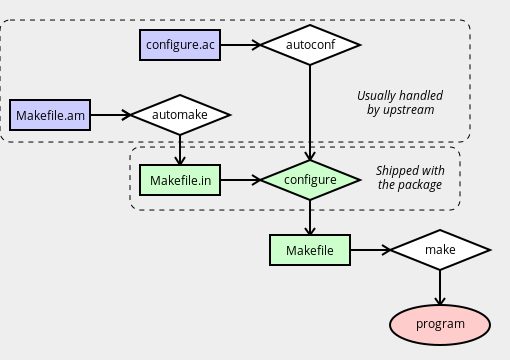
\includegraphics[width=12cm]{images/diagram.png}
	\caption{A basic overview of how the main Autotools components fit together.}
	\label{diagram}
\end{figure}
\vspace{2mm}

\section{\label{sec:dev-env}Set up Your Development Environment}

\justifying
The dev environment can be configured using the ``bootstrap.sh'' script and GNU autotools. This process should work well in Linux or Mac environments. There is also a development container that you can build if you are having
issues configuring these, wish to run in a different Operating System, etc.

\subsection{\label{sec:dev-linux}Option 1: Set up on Linux and Mac}

\justifying
\begin{raggedright}
    \begin{enumerate}
        \item Clone the Github repository from \href{https://github.com/devsecfranklin/workshop-codemash-2023}{https://github.com/devsecfranklin/workshop-codemash-2023}.
        \item In the newly created ``workshop-codemash-2023'' directory, execute the ``bootstrap.sh'' script.
        \item Next, run the ``./configure'' command.
        \item Finally, run the ``make python'' command to prepare the necessary Python modules.
    \end{enumerate}
\end{raggedright}
\vspace{2mm}

\subsection{\label{sec:dev-container}Option 2: Set up the dev Container}

\justifying
\begin{raggedright}
    \begin{enumerate}
        \item Create a new Github account using the second e-mail address.
        \item As your ``main user'', invite the bot user ``bot-account'' as a collaborator on the repo.
        \item Add the Github action to the repository.
    \end{enumerate}
\end{raggedright}
\vspace{2mm}

\section{\label{sec:github}Github Setup}


\justifying
\begin{raggedright}
	\begin{enumerate}
		\item Create a new Github account using the second e-mail address.
		\item As your ``main user'', invite the bot user ``bot-account'' as a collaborator on the repo.
		\item Add the Github action to the repository.
	\end{enumerate}
\end{raggedright}
\vspace{2mm}

\justifying
You can add a cool icon to the bot account Github profile.

\markdownInput{code/cloudbotyaml.md}

\section{\label{sec:Python}Python}

\justifying
The Python code is meant to run as a ``Cloud Function'' in GCP. This is a cost-effective way to run code
without deploying cloud infrastructure such as dedicated host instances or other cloud infrastructure
that must be maintained. We get to run our code and let Google take care of the rest.

\section{\label{sec:Terraform}Terraform}

\section{\label{sec:next}Going a Bit Further}

\justifying
This optional section describes how you can connect your Cloud Function to your Kubernetes cluster to extend the functionality even more.

\section{\label{sec:cleanup}Cleanup}

\justifying

docker system prune


\clearpage
\begin{versionhistory}
	\vhEntry{v0.1}{October 2nd, 2022}{Franklin Diaz}{Initial Draft}
\end{versionhistory}

\clearpage
% \nocite{*}
\bibliographystyle{plain}
\bibliography{mybib.bib}

\end{document}
